% =====================================================================================
%  Section 4.6 — What explains the improvement?
%  Self-contained. Nothing to \input.
%
%  PREAMBLE (already in main.tex): graphicx, booktabs, multirow, threeparttable
%  ASSETS: figures/fig_matched_control.pdf, figures/fig_aliasing.pdf
%    Regenerate both:  PYTHONPATH=. python -m experiments.make_fig_mechanism
%
%  DO NOT SOFTEN THE ALIASING SUBSECTION. It reports a prediction this project made and then
%  refuted with its own data, and it records that the prediction was written down before the
%  planner figure was computed. That ordering is what makes it evidence rather than a
%  rationalisation, and it is worth more to the examiner than a result that merely worked.
% =====================================================================================

\section{What Explains the Improvement?}\label{sec:res:mechanism}

Section~\ref{sec:res:internalise} showed that distilling the shielded policy's own clean rollouts
makes it dramatically safer without the shield. It does not, on its own, establish \emph{why}. The
demonstrations were filtered on three properties at once --- the shield fired, the episode
succeeded, and nothing was displaced --- and two mechanisms are bundled inside that filter.

Under the first, \textbf{distillation}, the policy imitates the shield's avoidance corrections.
This is the claim of this work. Under the second, \textbf{selection}, the improvement comes from
training a policy on its own successful episodes, a known self-improvement effect requiring no
shield at all; successful episodes also happen to be the ones in which nothing was knocked over. If
the second mechanism accounts for the result, the shield is incidental and the contribution is a
rediscovery of filtered behaviour cloning.

Nothing in the six-condition evaluation of Section~\ref{sec:res:internalise} distinguishes them, so
a matched control was run.

\subsection*{The matched control}

Demonstrations were collected with the shield \textbf{switched off}, filtered by exactly the same
criteria --- succeeded and displaced nothing --- and used to train a student with identical
hyperparameters. The shielded pool was then subsampled to the same size, so the two conditions
differ in one respect only: whether the shield was active while the demonstrations were being
generated.

\begin{table}[htbp]
\centering
\caption{The matched control. Both distilled conditions use 85 demonstrations passing an identical
  filter; they differ only in whether the shield was active during collection. $n = 120$ held-out
  rollouts per row, Wilson 95\% intervals.}
\label{tab:matched_control}
\begin{tabular}{lccc}
\toprule
\textbf{Condition} & \textbf{Demos} & \textbf{TSR (95\% CI)} & \textbf{Collision (95\% CI)} \\
\midrule
Undistilled base & ---            & 58.3\% [49.4, 66.8] & 82.5\% [74.7, 88.3] \\
Control, shield \textbf{off}  & 85 & 50.0\% [41.2, 58.8] & 84.2\% [76.6, 89.6] \\
Matched, shield \textbf{on}   & 85 & \textbf{75.8\% [67.4, 82.6]} & \textbf{26.7\% [19.6, 35.2]} \\
\bottomrule
\end{tabular}
\end{table}

\begin{figure}[htbp]
  \centering
  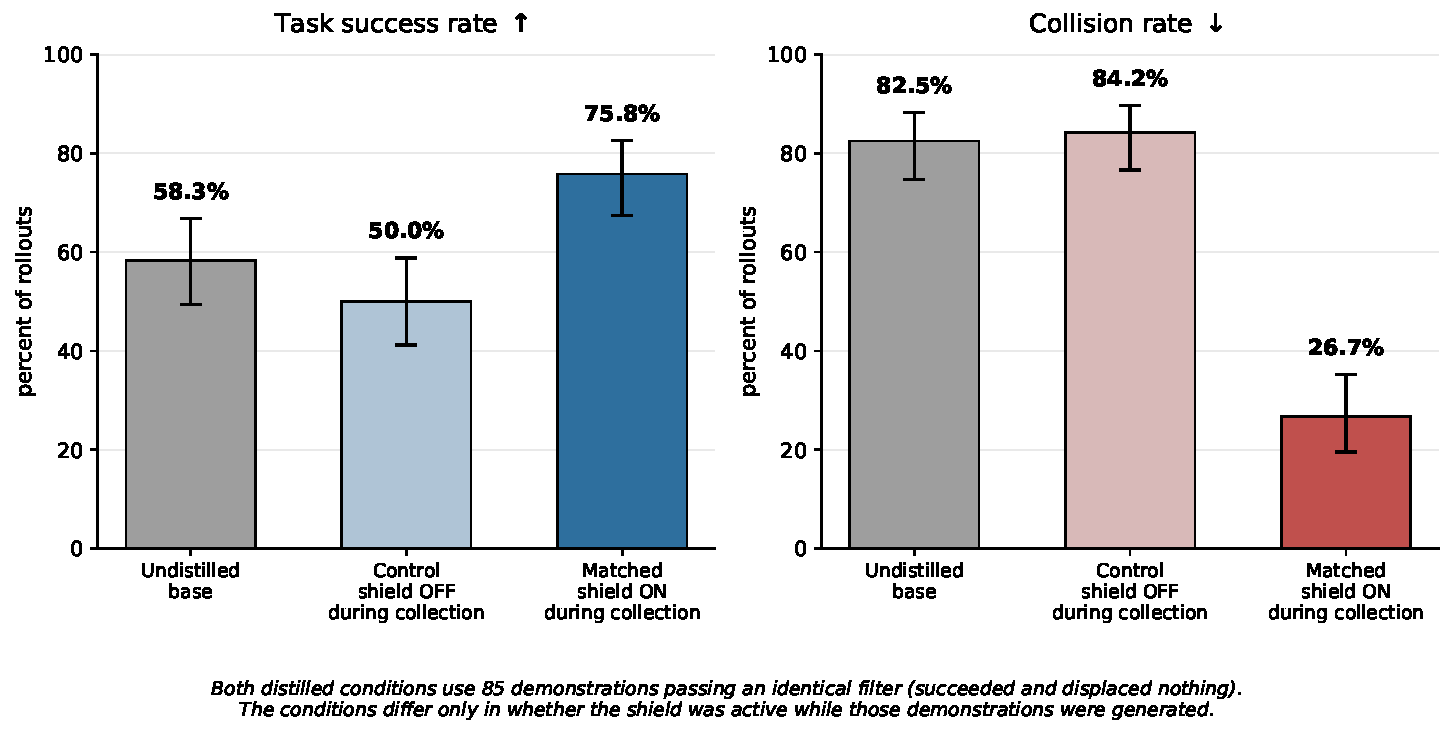
\includegraphics[width=\linewidth]{figures/fig_matched_control.pdf}
  \caption[The matched control: selection versus correction]{%
    Separating selection from correction. Training on the policy's own successful, collision-free
    episodes (centre) leaves it indistinguishable from the undistilled baseline. Applying the same
    filter to demonstrations collected while the shield was active (right) produces the effect.
    Since the two distilled conditions use the same number of demonstrations, the same filter and
    the same hyperparameters, the difference is attributable to the shield.}
  \label{fig:matched_control}
\end{figure}

\paragraph{Success-filtering alone achieves nothing.}
The control sits at 84.2\% collision, statistically indistinguishable from the undistilled base
policy at 82.5\%. Training a policy on its own successful, collision-free episodes did not make it
safer on this benchmark.

\paragraph{The shield's corrections are what transfers.}
At the same demonstration count and under the same filter, the shielded condition reaches 26.7\%,
with a confidence interval disjoint from the control's. The difference between the two conditions
is attributable to the shield and to nothing else in the pipeline. This is the experiment that
answers the most natural objection to Section~\ref{sec:res:internalise}, and it answers it directly
rather than by argument.

\paragraph{Two further pieces of evidence.}
The conclusion is corroborated by two measurements taken for other purposes. First, the CBF
activation proxy falls from 0.533 to 0.265 between the shielded base and the shielded distilled
policy: after distillation the shield finds materially less to correct. Success-filtering alone
does not predict this --- a policy that merely completes tasks more often would not require
\emph{less} safety intervention. Second, the demonstrations are pervasively shield-shaped, with the
barrier active on a median 32\% of control steps and a mean correction norm of 0.33 against actions
bounded at $\pm 1$, so the imitated action distribution differs substantially from the base
policy's own.

\paragraph{A nuance worth preserving.}
The control is not uniformly inert. Its per-body attribution shows arm-link collisions falling from
17 to 6 while gripper collisions remained high at 44, which is why the total did not move. Outcome
selection therefore \emph{does} transfer avoidance in the channel the barrier cannot express ---
exactly the second transfer channel identified in Section~\ref{sec:res:scope} --- but it is not
sufficient on its own. The two mechanisms are complementary rather than competing, and only one of
them addresses the end-effector channel that dominates the collision count.

\paragraph{The cost of collecting without a shield.}
One further number deserves reporting. The unshielded collection retained 85 usable demonstrations
from 480 rollouts, a yield of 18\%, against 39\% for the shielded collection. Safe demonstrations
are roughly twice as expensive to obtain without a shield. This is a second, independent sense in
which the shield earns its place: beyond supplying the corrections that transfer, it makes the
collection of a safe demonstration set tractable in the first place.

\subsection*{Two alternative explanations tested and rejected}

Section~\ref{sec:res:source} established that distilling from a foreign expert fails while
self-distillation succeeds. Two explanations for that boundary were tested directly, and both were
rejected.

\paragraph{Observation aliasing.}
Earlier analysis in this project attributed the failure to the policy's observation space:
$\pi_{0.5}$ sees an image and eight proprioceptive dimensions, with no joint angles, so a
correction depending on the full arm configuration is not a function of anything the policy
observes, and behaviour cloning would average contradictory targets. This was asserted but never
measured, and it is measurable from the demonstration files alone. For each dataset, samples whose
observations are near neighbours were found and the disagreement between their target actions
measured, normalised by the disagreement between random pairs. Comparison is made at matched
observation \emph{radius} rather than matched neighbour count, because a nearest-neighbour ratio
conflates aliasing with sampling density and the planner's trajectories are far denser.

\begin{figure}[htbp]
  \centering
  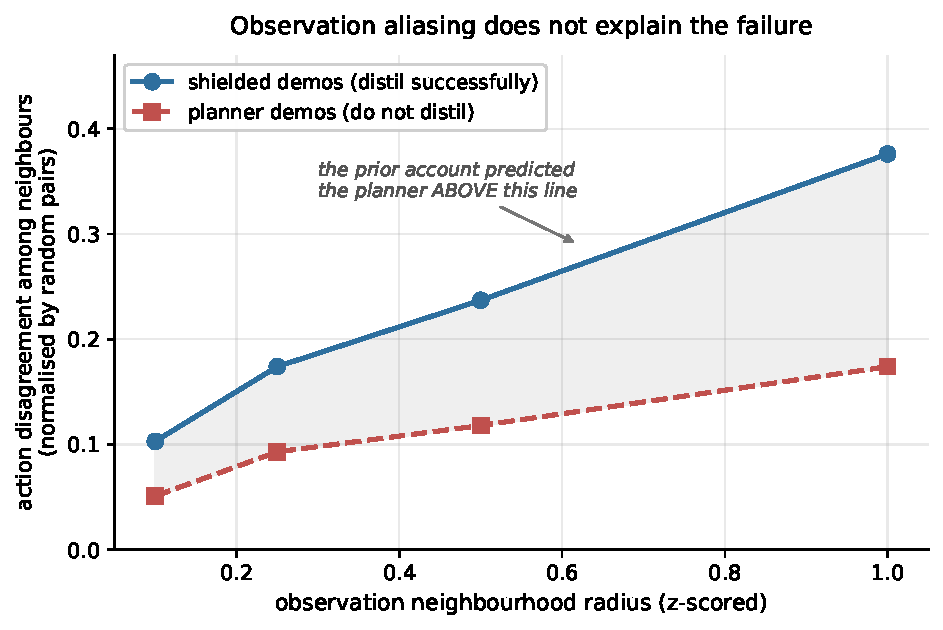
\includegraphics[width=0.72\linewidth]{figures/fig_aliasing.pdf}
  \caption[Observation aliasing does not explain the transfer failure]{%
    A prediction of this project, refuted by its own data. If the planner's corrections were
    poorly determined by what the policy observes, its curve would lie \emph{above} the shielded
    one. It lies consistently below, by a factor of roughly two at every radius: the teacher that
    fails to distil has the cleaner observation-to-action mapping.}
  \label{fig:aliasing}
\end{figure}

\begin{table}[htbp]
\centering
\caption{Action disagreement among observation-neighbours, normalised by random-pair disagreement.
  Lower values mean the action is better determined by the observation.}
\label{tab:aliasing}
\begin{tabular}{lcc}
\toprule
\textbf{Radius (z-scored)} & \textbf{Shielded (distils)} & \textbf{Planner (does not)} \\
\midrule
0.10 & 0.103 & 0.051 \\
0.25 & 0.174 & 0.093 \\
0.50 & 0.237 & 0.118 \\
1.00 & 0.376 & 0.174 \\
\bottomrule
\end{tabular}
\end{table}

The ordering is the reverse of the prediction. The planner's demonstrations are roughly twice as
\emph{well} determined by the observation at every radius: the teacher that fails to distil has the
cleaner observation-to-action mapping, and the teacher that succeeds is the more aliased of the
two. In hindsight the direction is unsurprising --- a scripted planner is close to a deterministic
function of state --- but it means aliasing is not the binding constraint, and the prior
explanation does not survive contact with the data. The prediction was recorded before the planner
figure was computed. The surviving candidates are distribution shift and action-distribution
mismatch, and Section~\ref{sec:res:source} takes up the first of them.

\paragraph{Generative uncertainty as a collision predictor.}
$\pi_{0.5}$ produces each action by integrating a flow ordinary differential equation, and every
rollout stores that denoising chain. If the policy were less certain in states where safe and
unsafe behaviours are both plausible, the chain geometry would carry a risk signal, and a runtime
monitor could use it with no barrier and no obstacle geometry. Scored as the area under the ROC
curve for predicting whether an episode collided, the result is negative: 0.461 for the base
policy, which is chance. The distilled policy shows a consistent inverted association across all
three chain statistics (AUC 0.350, equivalently 0.65 when flipped, so \emph{lower} uncertainty is
associated with collision), but on 23 collision episodes that is roughly two standard errors from
chance and far short of deployable. The suggestive reading, if it is real, is that the distilled
policy's failures are \emph{confident} ones, which would make uncertainty-based monitoring
structurally unsuited to this failure mode.
